\chapter{Simulator GUI}\label{sec:simulator_pictures}
User controls are provided for managing environment time, choosing presets and protocols, and accessing statistics. The graphical view, which has full support for panning and zooming, displays the environment's: objects, radios and transmissions. 

Objects are drawn using their obstruction shape (and specified attributes).  Radios are drawn as blue circles when transmitting and grey circles otherwise. Transmission routes are displayed for the last received data in a radio's buffer as a line from transmitter to receiver with \ac{snr} indicated; preamble is identified by a dotted line, payload as a solid line. The line will be grey if the receiver failed to synchronise with the preamble or red if the transmission was not the one the receiver is synchronised with (Figure \ref{fig:sim_view_interference}). Otherwise, blue is used to indicate a data packet and orange as protocol overhead (Figure \ref{fig:sim_view_overhead}). Together visual cues provides an exact understanding of the system behaviour.

As the system can execute quicker than the view can update, it can optionally be buffered such that system execution runs only as fast as the view updates. Selecting a radio will allow it to be moved, even if it is transmitting. Along with \ac{rssi}s this allows quick verification of how noise patterns in a network can be effected by transmissions. The toggle for showing all routes shows potential routes if a radio were to transmit (Figure \ref{fig:sim_view_all_routes}); this means radios on matching configurations are joined. These routes will be red if they cannot communicate but still interfere (e.g. same chirp rate and frequency but different \ac{sf}).


\begin{figure}[H]
    \centering
   	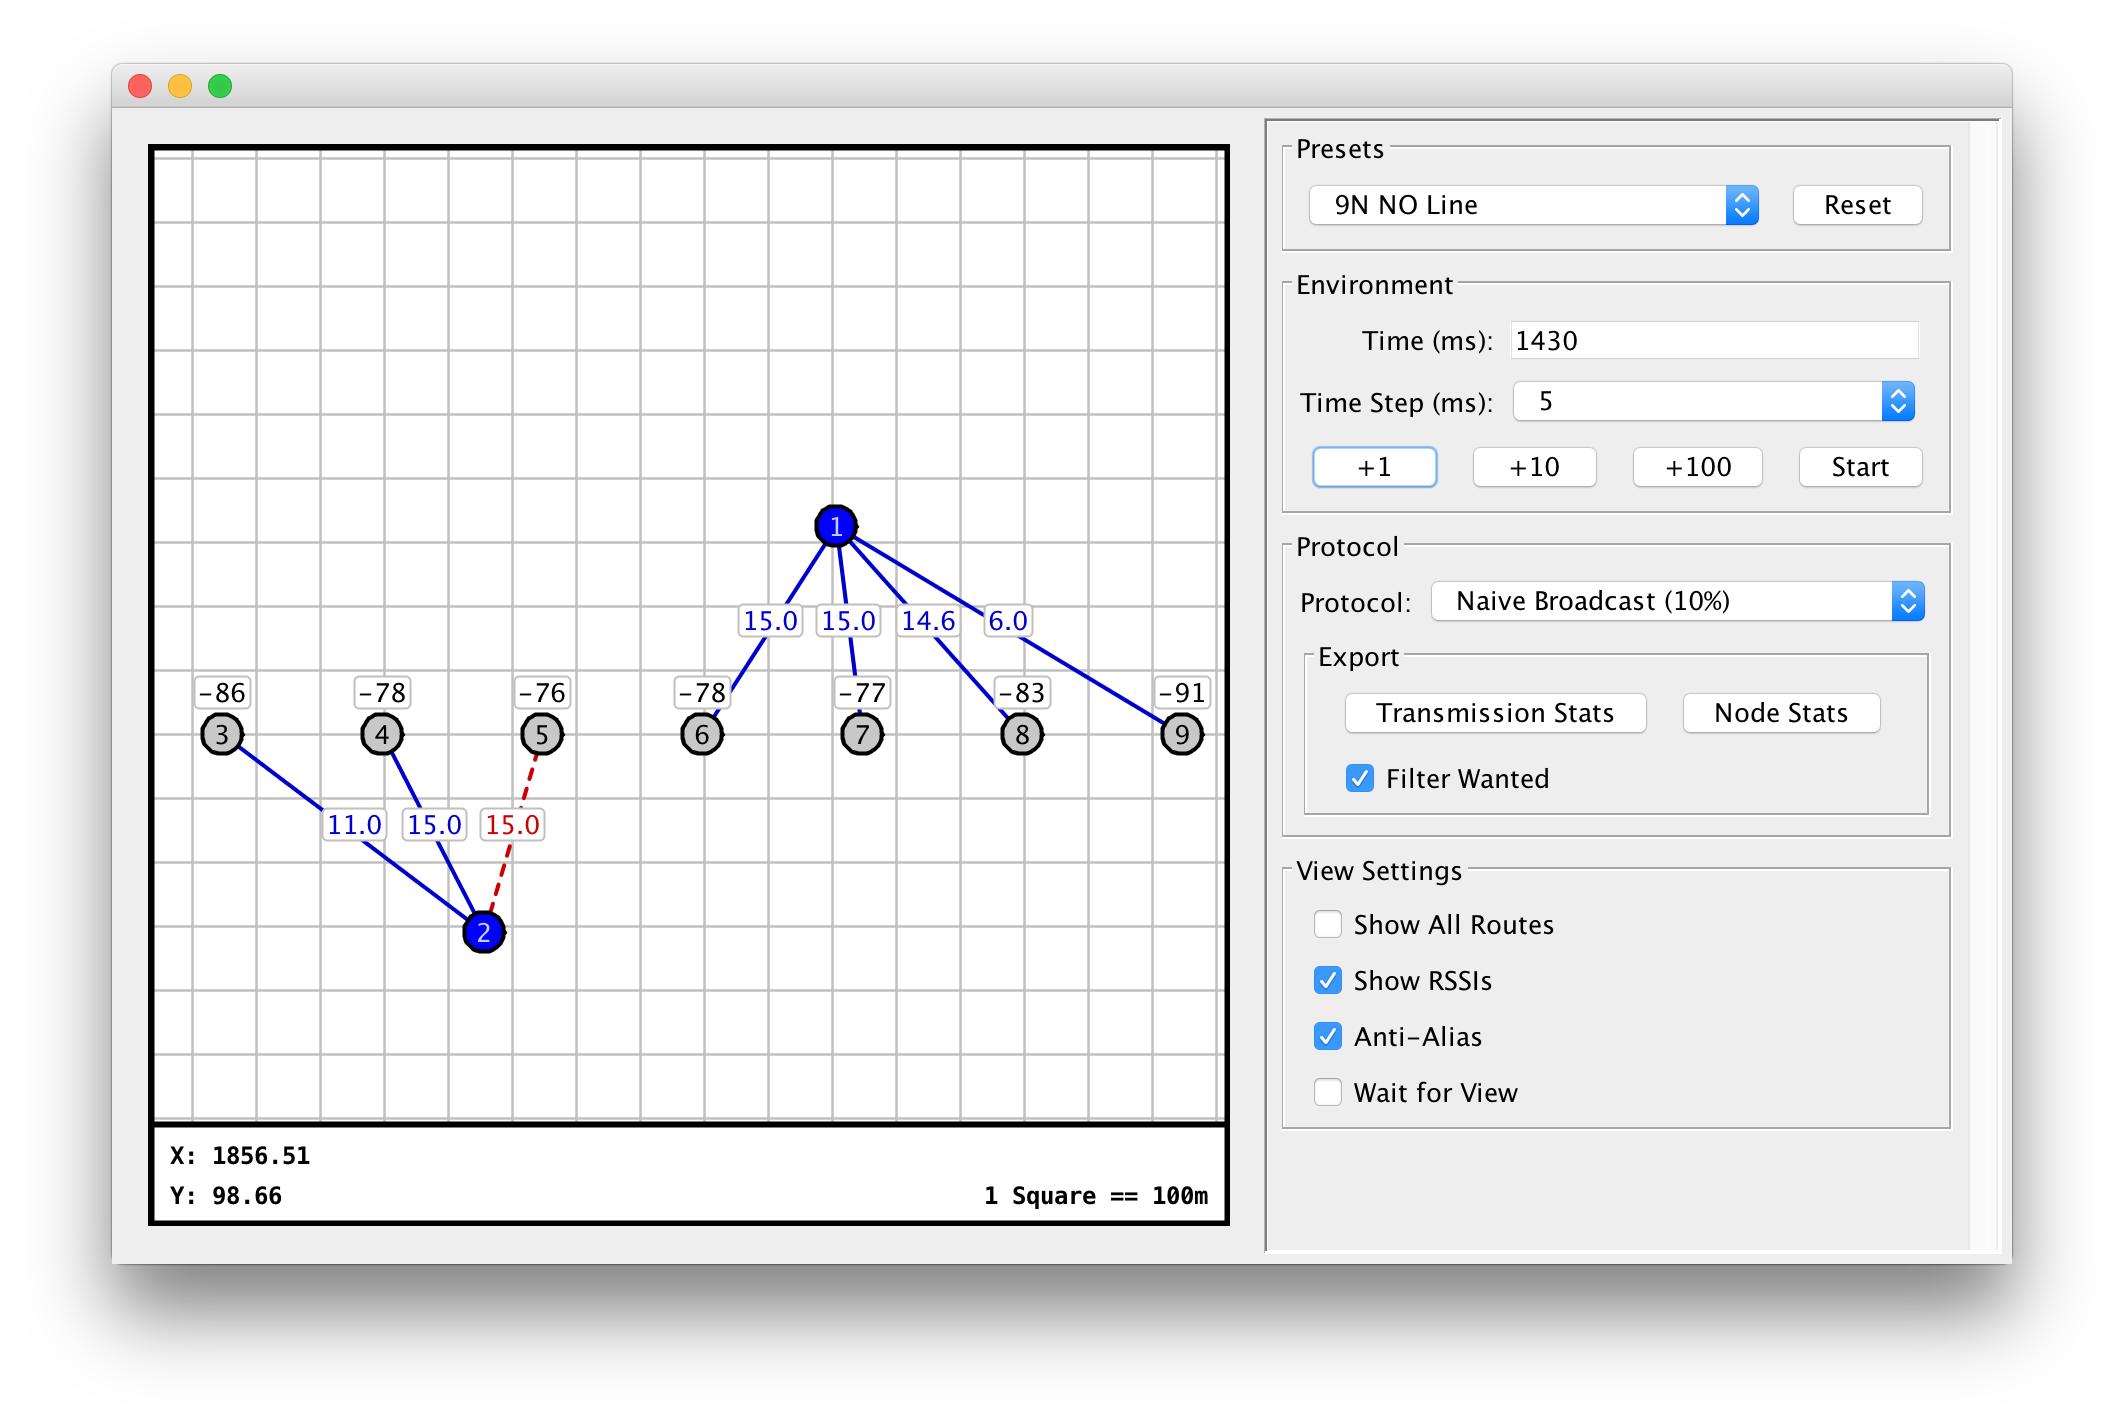
\includegraphics[width=\textwidth]{Figures/simulator_interference}
    \caption[Simulator view with interference]{
    	Simulator view when a stronger transmission (from 2) has started after a receiver (5) has already synchronised with a transmission (from 1).
    	\label{fig:sim_view_interference}
    }
\end{figure}

\begin{figure}[H]
    \centering
   	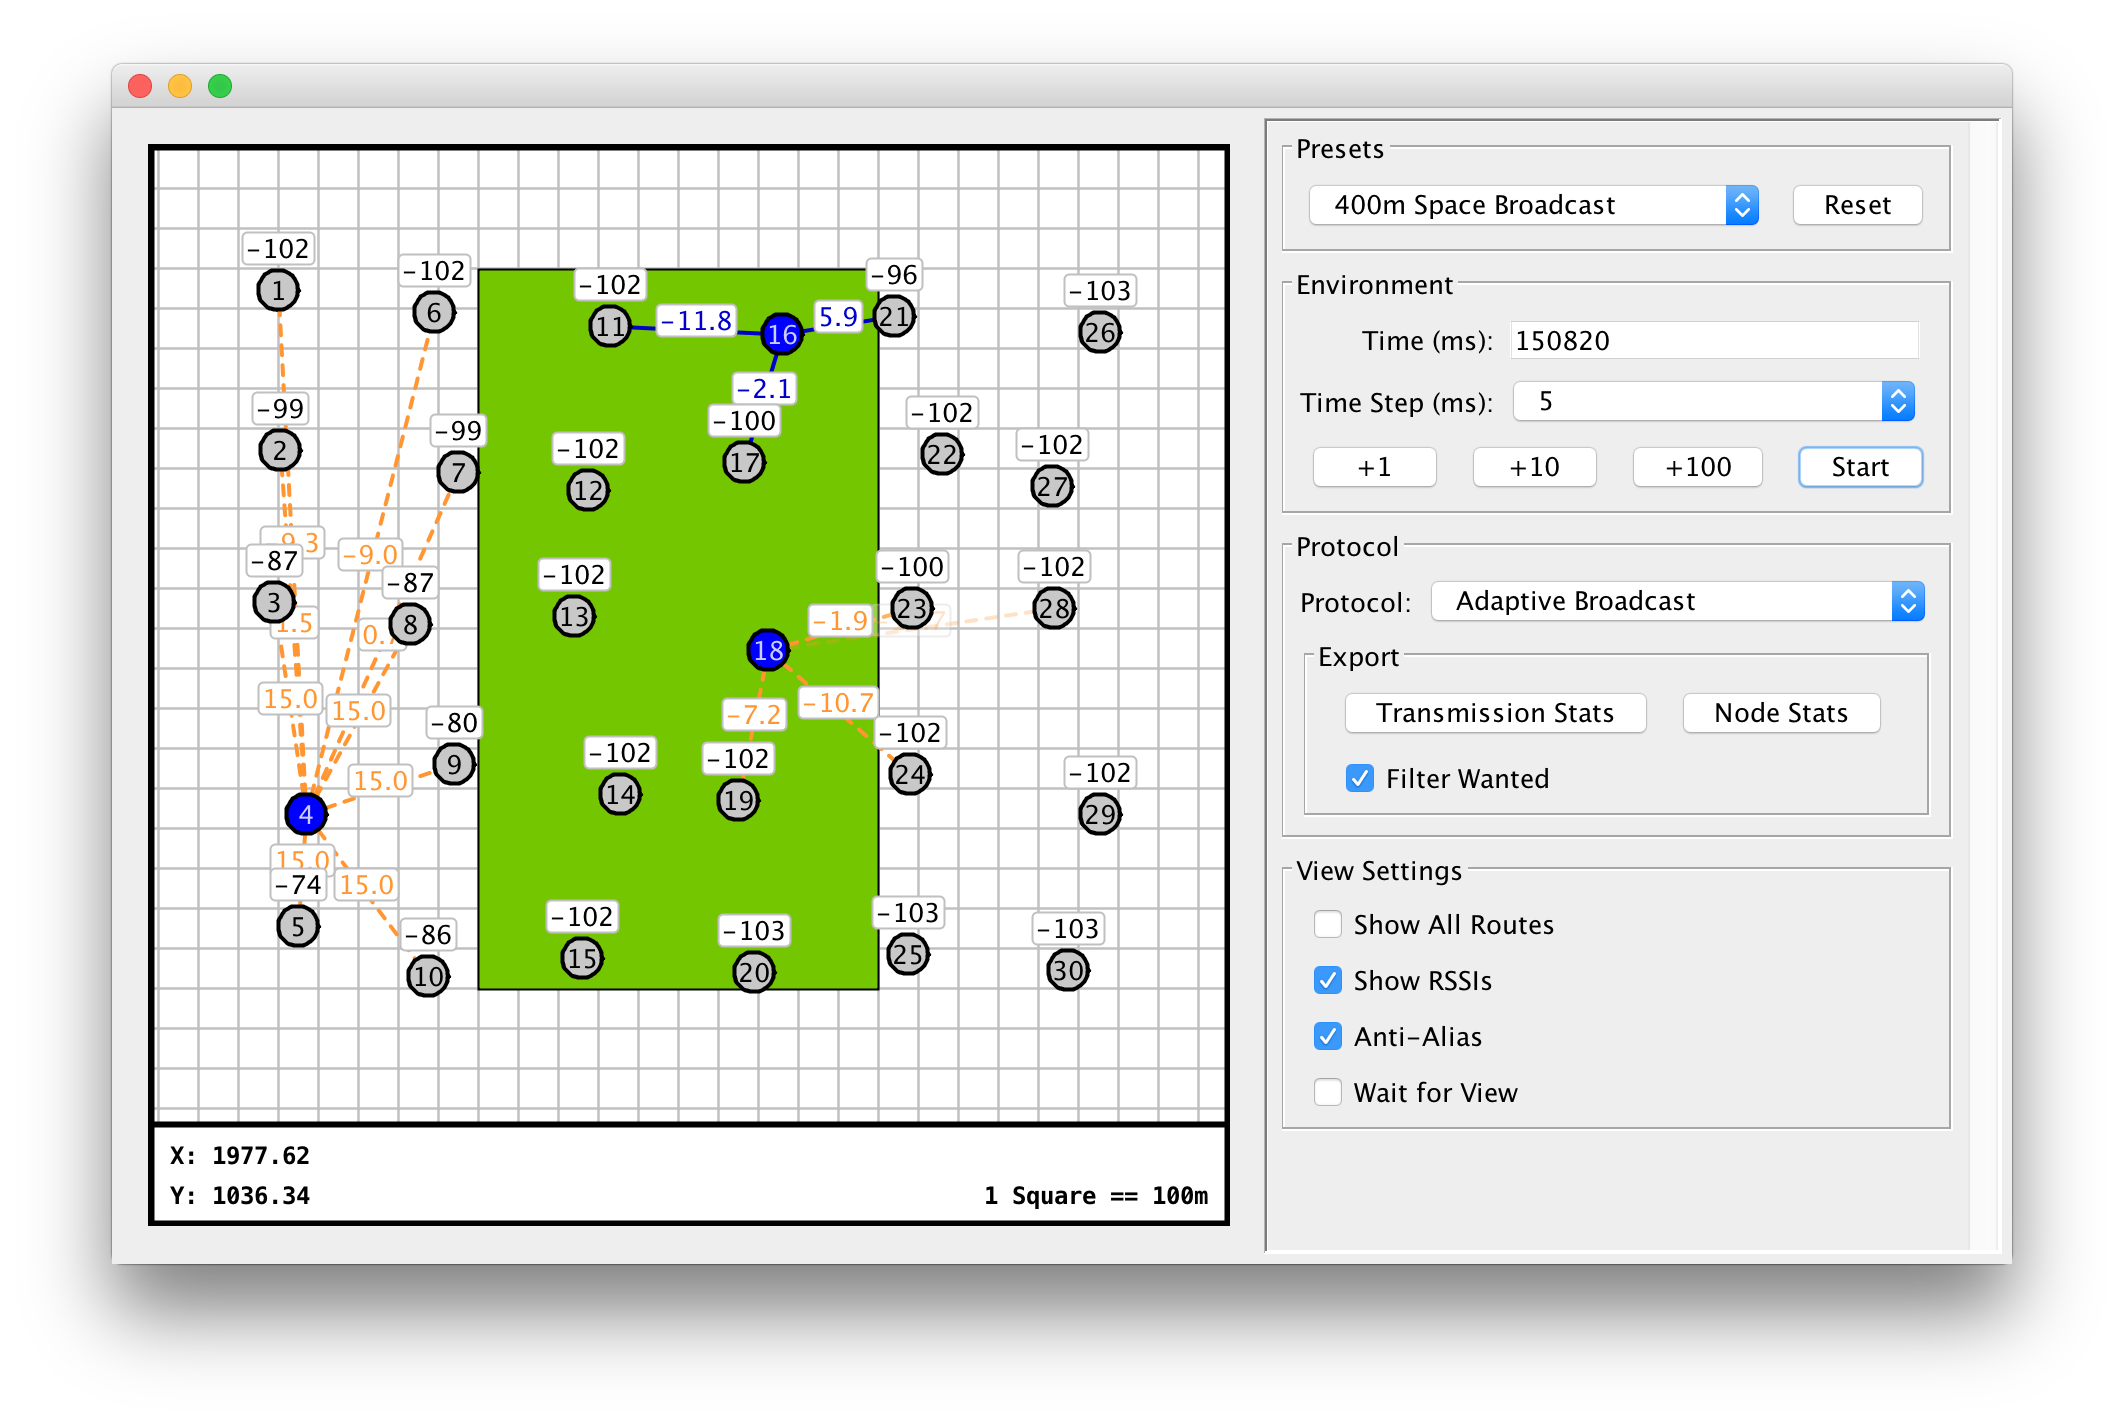
\includegraphics[width=\textwidth]{Figures/simulator_overhead}
    \caption[Simulator view with data and overhead]{
    	Simulator view when some transmissions are protocol overhead packets, whilst others are data packets.
    \label{fig:sim_view_overhead}
    }
\end{figure}

\begin{figure}[H]
    \centering
   	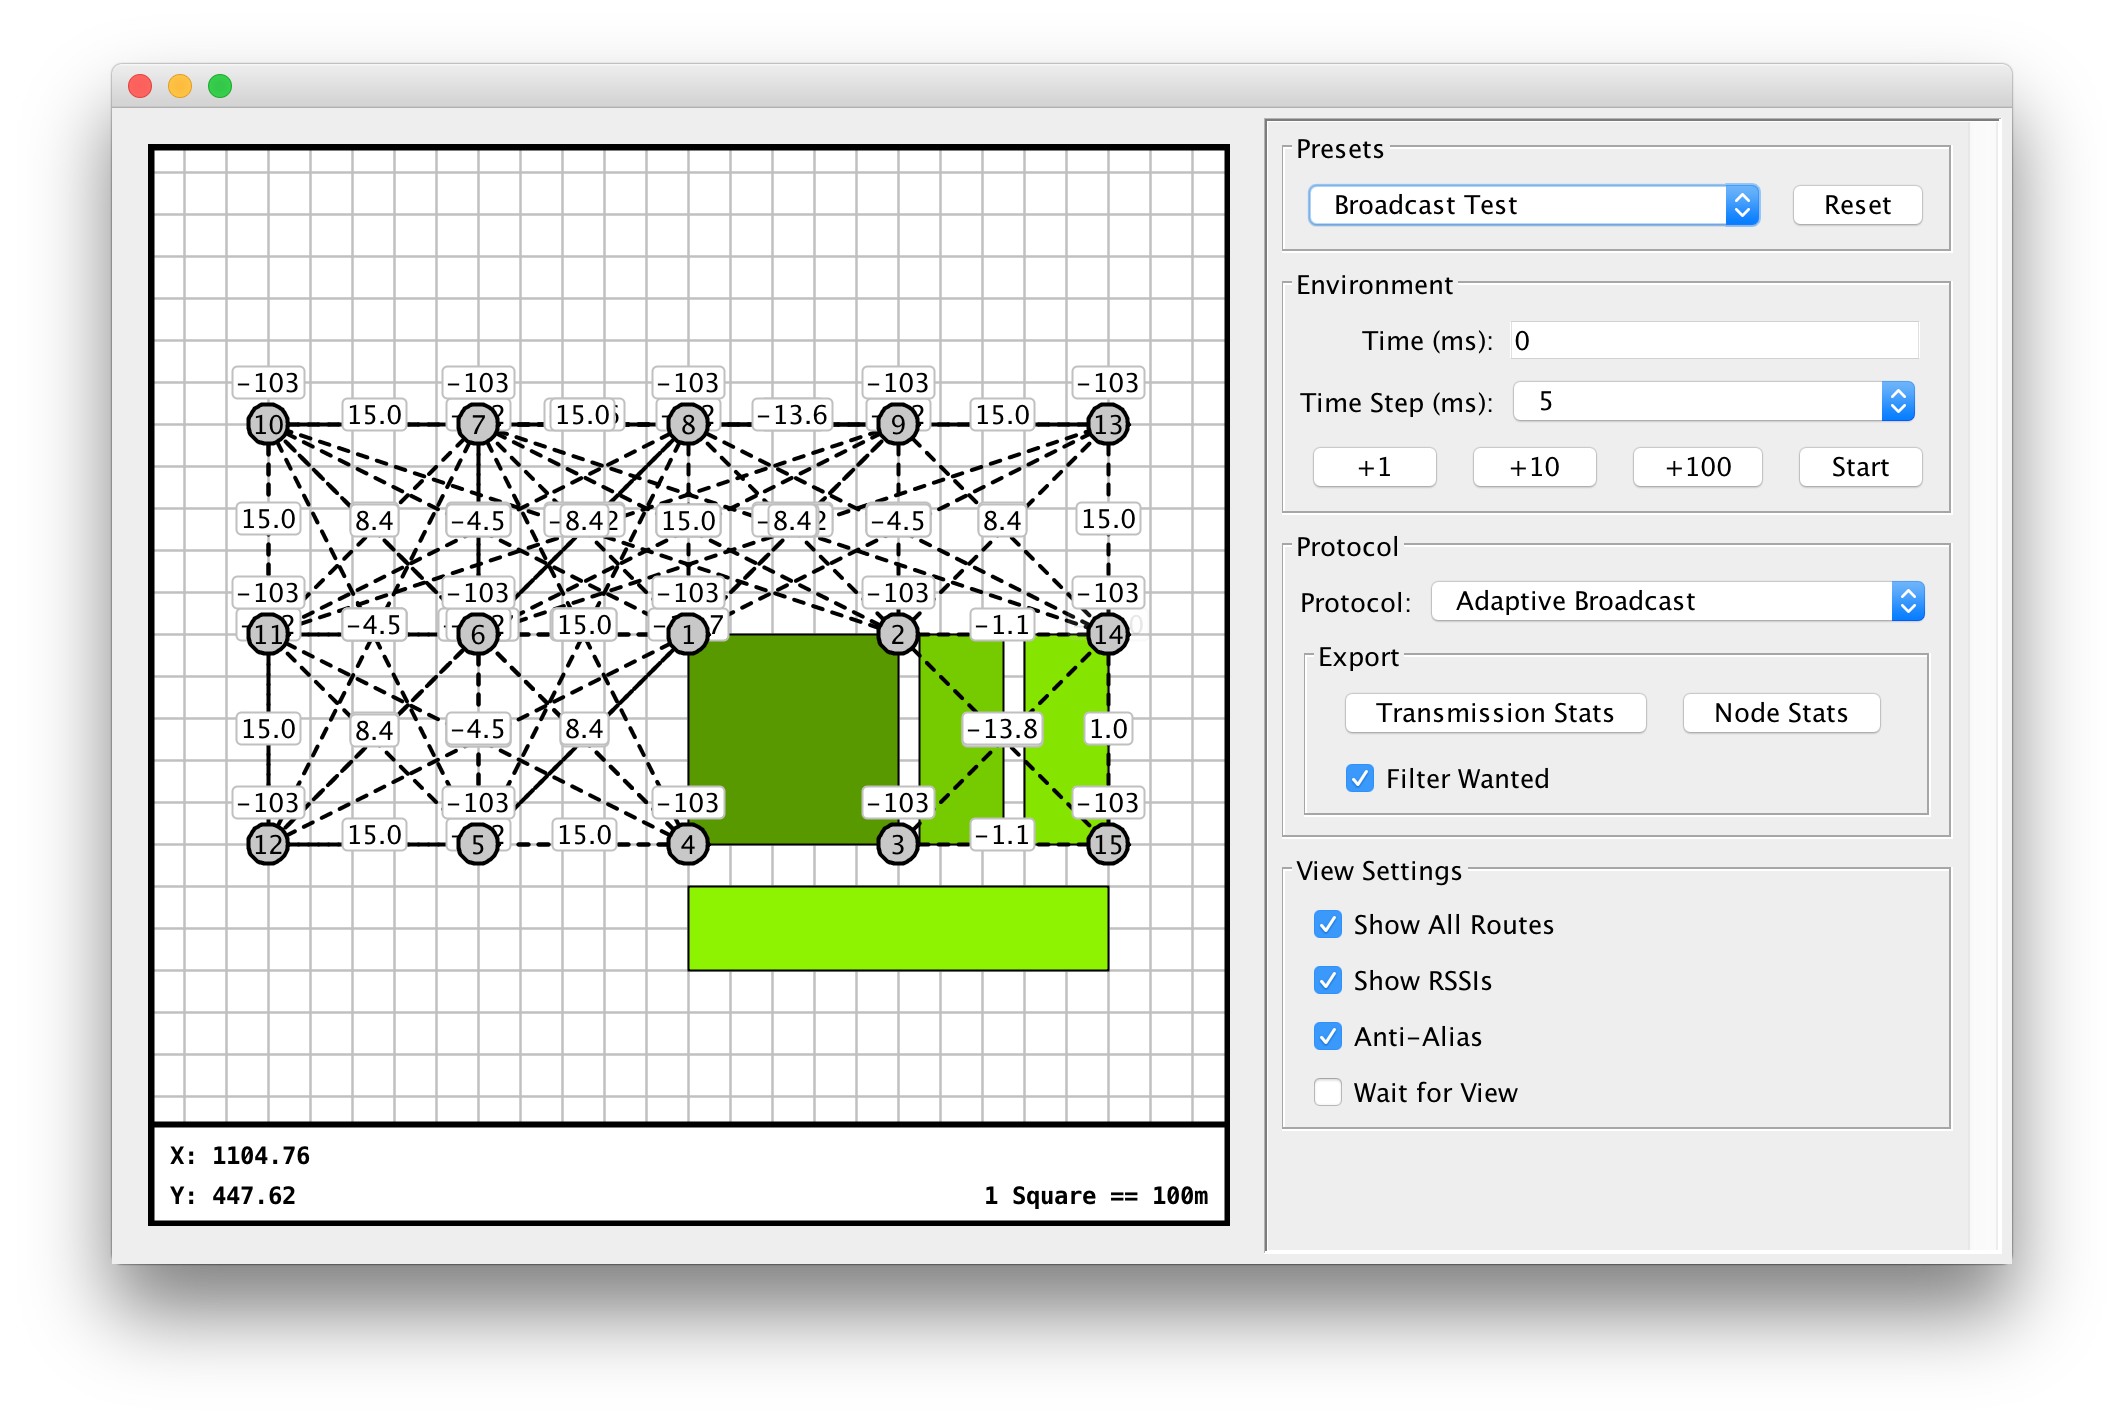
\includegraphics[width=\textwidth]{Figures/simulator_all_routes}
    \caption[Simulator view with all routes shown]{
    	Simulator view when all potential receivable routes are being shown. No transmissions are actually occurring.
   	\label{fig:sim_view_all_routes}
    }
\end{figure}